\documentclass[11pt,a4paper]{article}
\usepackage[margin=2.3cm]{geometry}
\usepackage[T1]{fontenc}
\usepackage{lmodern}
\usepackage{amsmath,amssymb}
\usepackage{graphicx}
\usepackage{booktabs}
\usepackage{tabularx}
\usepackage{array}
\usepackage{xcolor}
\usepackage{tikz}
\usetikzlibrary{arrows.meta,positioning,calc}
\usepackage{caption}
\usepackage{subcaption}
\usepackage{float}
\usepackage{enumitem}
\usepackage[hidelinks]{hyperref}
\setlist{nosep,leftmargin=*}
\emergencystretch=3em
\graphicspath{{../docs/screenshots/}}
\definecolor{cause}{HTML}{2A78D6}
\definecolor{decoy}{HTML}{EB6834}
\newcolumntype{L}{>{\raggedright\arraybackslash}X}
\newcolumntype{P}[1]{>{\raggedright\arraybackslash}p{#1}}
\tikzset{
  n/.style={draw, rounded corners=3pt, align=center, font=\small, inner sep=4pt, fill=gray!8},
  hid/.style={n, dashed, fill=white},
  cs/.style={n, draw=cause, very thick, fill=cause!12},
  dc/.style={n, draw=decoy, thick, fill=decoy!12},
  outc/.style={n, fill=black, text=white},
  ar/.style={-{Stealth[length=2.2mm]}, thick, gray!70!black},
  arc/.style={-{Stealth[length=2.6mm]}, line width=1.4pt, cause},
  arr/.style={-{Stealth[length=2.4mm]}, line width=1.2pt, decoy},
  sp/.style={dotted, line width=1.2pt, decoy},
  lab/.style={font=\scriptsize\itshape, text=black!70}
}

\title{\textbf{Mayor for a Year}\\[4pt]\large A simulation game for learning that correlation does not imply causation}
\author{Rohan Karthik K (EC24B1015) \and Vasanth M S (EC24B1059)\\[4pt]
\small CS3006 Introduction to Data Science, Part B: Game for learning data science concepts\\
\small Indian Institute of Information Technology, Design and Manufacturing, Kancheepuram}
\date{November 2026}

\begin{document}
\maketitle

\begin{abstract}
\noindent \emph{Mayor for a Year} is a browser game in which the player governs a fictional Indian town and must
fix one public problem per level using a budget and a dashboard of the town's data. Each level is driven by a hidden
structural causal model (SCM) whose data contains a deliberate trap: the most tempting correlation does not point at
the cause. The player explores the data, funds one policy, watches the next season simulated twice (with and without
the policy, using common random numbers), and is then shown the hidden causal diagram. Five levels cover confounding,
reverse causation, Simpson's paradox and randomised experiments, each unlocking a new analysis tool; the final level
tests transfer with new stories under a shared budget. Every world is generated afresh from a seed, every statistic is
computed live, and 44 automated tests verify that the traps hold, that interventions on non-causes have exactly zero
effect, and that the in-game randomised pilot is unbiased with near-nominal confidence-interval coverage. The game logs
every decision, includes a pre/post scenario quiz and a feedback form, and ships with a script that turns players' logs
into a playtest summary.
\end{abstract}

\section{Introduction}
``Correlation does not imply causation'' is one of the first warnings in any data science course, and also one of the
easiest to agree with and then ignore. Reading the slogan does not teach a learner \emph{why} a correlation misleads,
\emph{which} mechanism is at work, or \emph{what to do} about it. Our aim was a game in which the learner discovers these
ideas by acting on data and seeing the consequences, rather than by reading about them or answering questions.

The design rests on one observation: in a simulation we know the true causes, so we can show a player the real effect of
their decision. A player who bans ice-cream because ice-cream sales track dengue can be shown, in the same simulated
season, that dengue was exactly as bad as it would have been. That gap between ``what the data suggested'' and ``what
actually happened'' is the learning moment the game is built around.

\section{Concept and learning objectives}
The game teaches one concept, \textbf{correlation does not imply causation}, through four mechanisms, each the subject of
one level. After playing, a learner should be able to:
\begin{enumerate}
  \item explain why a strong correlation does not show causation;
  \item recognise confounding, reverse causation and Simpson's paradox in data;
  \item use stratification (comparing like with like) to control for a confounder;
  \item explain why randomised experiments establish causation.
\end{enumerate}
These objectives are shown on the start screen. Table~\ref{tab:objectives} maps each objective to the level that teaches it
and to the evidence the game records.

\begin{table}[H]
\centering\small
\caption{Learning objectives, where they are taught, and how learning is measured.}
\label{tab:objectives}
\begin{tabularx}{\textwidth}{@{}P{3.7cm}LL@{}}
\toprule
Objective & Taught by & Evidence recorded \\
\midrule
1. Correlation $\neq$ causation & Every level: the strongest correlate is never the best policy; the reveal table contrasts $r$ with simulated true impact & Trap-fall rate per level; quiz items 1--3 \\
2. Recognise the three traps & Level 1 (confounding), Level 2 (reverse causation), Level 3 (Simpson's paradox); Level 5 repeats them in new stories & Trap-fall in Level 5 vs Level 1; quiz items 1--2 \\
3. Stratification & Level 1 ward averages (season held fixed); Level 3 ``Split by group''; Level 4 shows its limit when the confounder is unobserved & Use of the key tool before deciding (logged) \\
4. Randomised experiments & Level 4 randomised pilot; Level 5 decides when a pilot is worth its cost & Pilots run; quiz item 3 \\
\bottomrule
\end{tabularx}
\end{table}

\section{Game design}
\subsection{Premise, goal and rules}
The player is the new mayor of Navapuram, a town of 20 wards. In each level the player receives a problem (for example,
an approaching dengue season), a budget (Rs.~40 lakh), last year's data for every ward and week, and a list of candidate
policies with costs. The goal is to fund the \emph{one} policy that most improves the town over the coming 12-week season
while spending as little as possible. The causal structure is hidden; only data is visible. An advisor character
(Dr.~Asha) narrates the brief, and a newspaper headline pushes the tempting but wrong conclusion, with the actual
correlation coefficient computed from that game's data.

\subsection{Core loop}
Each level follows the same loop: \textbf{brief} $\rightarrow$ \textbf{explore} $\rightarrow$ \textbf{decide} $\rightarrow$
\textbf{simulate} $\rightarrow$ \textbf{reveal}.
\begin{description}
  \item[Explore.] The player investigates with the tools unlocked so far: an animated cartoon town in which every icon is
  data-driven (mosquitoes over a ward = that ward's dengue cases), a ward heatmap with week-by-week and yearly-average
  modes, a time-series plot, a scatter plot with Pearson $r$ (per ward-week or per ward average), and a raw data table
  with CSV export.
  \item[Decide.] The player funds one policy at the policy desk. From Level~4 the player may first run a randomised pilot.
  \item[Simulate.] The coming season is simulated twice, with and without the policy, on the same random numbers. Two
  towns and a line chart animate side by side, so the true impact is seen directly.
  \item[Reveal.] The hidden causal diagram is drawn arrow by arrow, the trap is explained in two or three sentences using
  that game's numbers, and a table lists, for every policy, its correlation with the outcome next to its simulated true impact.
\end{description}

\begin{figure}[tbp]
\centering
\begin{subfigure}{0.49\textwidth}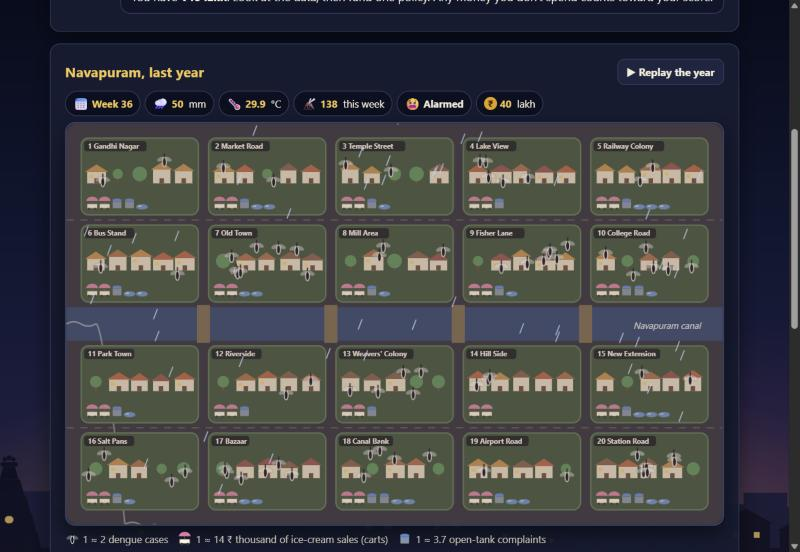
\includegraphics[width=\linewidth]{01_town.jpg}\caption{Explore: the living town (Level 1).}\end{subfigure}\hfill
\begin{subfigure}{0.49\textwidth}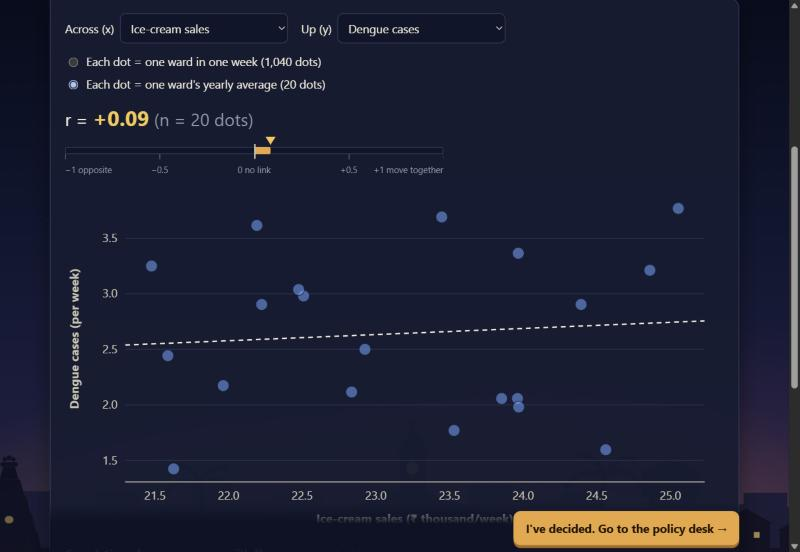
\includegraphics[width=\linewidth]{02_scatter_ward_averages.jpg}\caption{Explore: ward averages remove the season.}\end{subfigure}\\[4pt]
\begin{subfigure}{0.49\textwidth}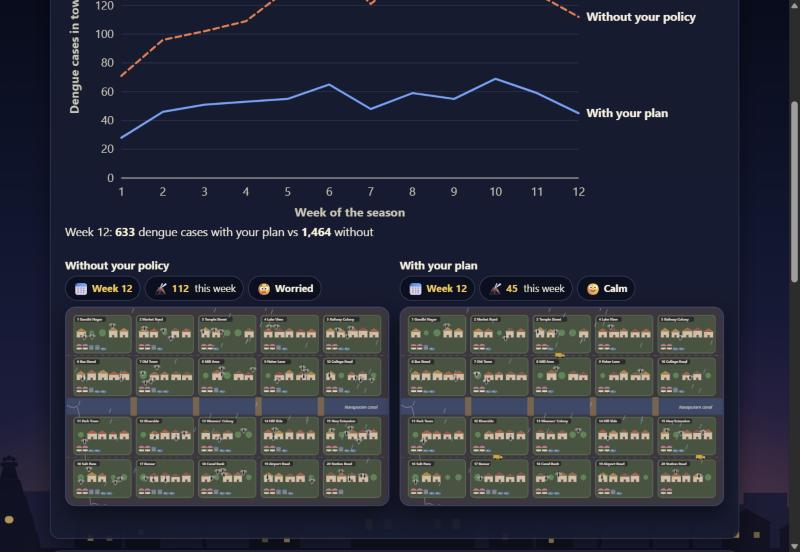
\includegraphics[width=\linewidth]{03_simulation.jpg}\caption{Simulate: with vs without, same luck.}\end{subfigure}\hfill
\begin{subfigure}{0.49\textwidth}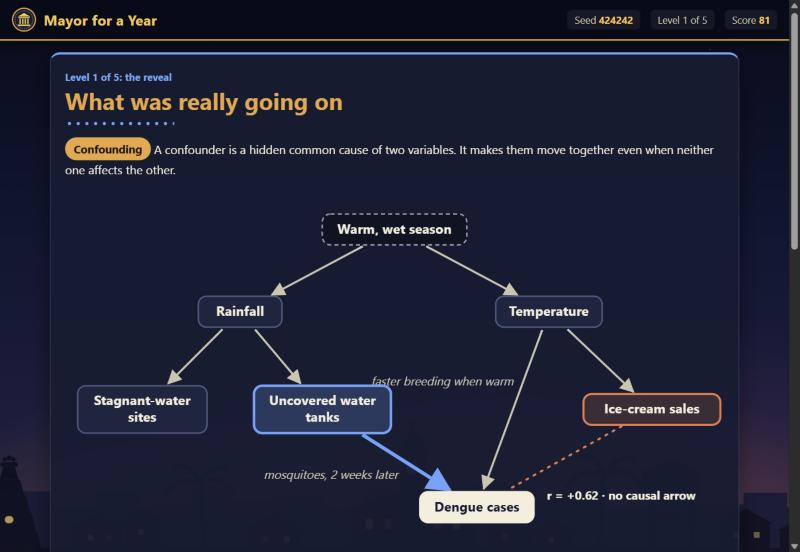
\includegraphics[width=\linewidth]{04_reveal.jpg}\caption{Reveal: the hidden causal diagram.}\end{subfigure}
\caption{The core loop of Level 1. In (b) ice-cream sales, the strongest ward-week correlate of dengue ($r=0.62$), show
no relation once wards are compared on yearly averages ($r=0.09$).}
\label{fig:loop}
\end{figure}

\subsection{Levels and progression}
Table~\ref{tab:levels} lists the five levels. Each introduces one mechanism and unlocks the tool that defeats it, so the
player's toolkit grows with the difficulty of the traps. Level~4 deliberately presents a confounder that is \emph{not} in
the data, so that no plot or split can resolve it and an experiment is the only reliable route. Level~5 contains three
problems with new stories and one shared budget of Rs.~90 lakh; running a pilot and a full roll-out on all three is
unaffordable, so the player must judge where the data already answers the question and where an experiment is worth its
cost. Because the stories are new, avoiding the traps here requires the idea, not a remembered answer.

\begin{table}[H]
\centering\small
\caption{Levels, traps and the tool each level unlocks.}
\label{tab:levels}
\begin{tabularx}{\textwidth}{@{}P{2.4cm}LLP{3.4cm}@{}}
\toprule
Level & Trap in the data & Mechanism & New tool \\
\midrule
1 Dengue season & Ice-cream sales are the strongest correlate of dengue & Confounding (season) & Town view, heatmap, time series, scatter + $r$, table \\
2 Clinic paradox & Wards with more clinics have more fever; closing clinics refunds money & Reverse causation & ``What changed first?'' (event study) \\
3 Coaching centres & Programme attenders score lower overall & Simpson's paradox & Class view, compare averages, split by group \\
4 Road accidents & All three road measures go with more accidents & Unobserved confounder & Randomised pilot, split by group \\
5 Final term & Diarrhoea vs cold drinks; thefts vs police posts; school absence & All of the above, transfer & All tools, shared budget \\
\bottomrule
\end{tabularx}
\end{table}

\subsection{Scoring and feedback}
For each problem the score out of 100 is
\begin{equation}
\text{score} = \max\!\Big(0,\; 70\,\frac{I}{I^{*}} \;+\; 30\,\frac{B - c}{B} \;-\; 20\,\frac{w}{B}\Big),
\end{equation}
where $I$ is the true impact of the player's plan, $I^{*}$ the best impact achievable by any single policy (found by
simulating every option), $B$ the budget, $c$ the money spent and $w$ the money spent on a policy whose impact is at most
5\% of $I^{*}$ (wasted spending). The ratio $I/I^{*}$ is clipped to $[-1,1]$, so a harmful policy loses points. Spending on
pilots counts against the budget but never as waste, because it buys information. Feedback is layered: the immediate gap
between the two simulated towns, the score breakdown, 0--3 stars, a newspaper headline written from the simulated outcome,
the advisor's reaction, and badges for good analysis habits (for example, ``Data detective'' for using the tool that
defeats that level's trap before deciding). Missed badges are shown with a hint, so each level tells the player what to try next time.

\subsection{Why this is a game and not a quiz}
The player never selects an answer to a question about causation. They act on a town, the town responds through a
simulation, and the consequence of the decision is visible and scored. The same choice can be right in one game and wrong
in another, because the roles of the candidate causes are shuffled. The optional pre/post quiz sits outside the game loop
and exists only to measure learning.

\section{Simulation model}
\subsection{Structural causal models}
Each level is a structural causal model: every variable is computed from its true causes plus independent noise, for
20 wards $\times$ 52 weeks of history (Level~3: 1{,}200 students). A policy is an intervention $do(X=x)$ that overrides
one equation. Figure~\ref{fig:dags} shows the four causal structures; the equations are summarised below, with
$S(t)$ a bell-shaped season curve, $e$ independent $N(0,1)$ noise and $w$, $t$ the ward and week.

\begin{figure}[H]
\centering
\begin{subfigure}[t]{0.49\textwidth}\centering
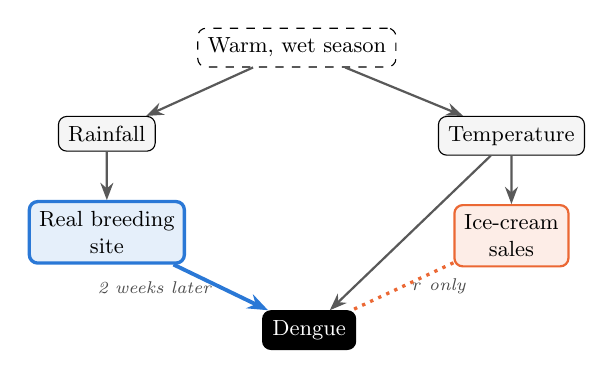
\begin{tikzpicture}[scale=0.88, transform shape, node distance=7mm and 6mm]
\node[hid] (s) {Warm, wet season};
\node[n, below left=of s] (r) {Rainfall};
\node[n, below right=of s] (t) {Temperature};
\node[cs, below=of r] (c) {Real breeding\\site};
\node[dc, below=of t] (i) {Ice-cream\\sales};
\node[outc,below=11mm of $(c)!0.5!(i)$] (d) {Dengue};
\draw[ar] (s)--(r); \draw[ar] (s)--(t); \draw[ar] (r)--(c); \draw[ar] (t)--(i); \draw[ar] (t)--(d);
\draw[arc] (c)--node[lab,left]{2 weeks later}(d);
\draw[sp] (i)--node[lab,right]{$r$ only}(d);
\end{tikzpicture}
\caption{Level 1: confounding.}\end{subfigure}\hfill
\begin{subfigure}[t]{0.49\textwidth}\centering
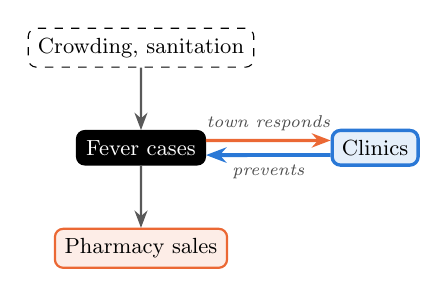
\begin{tikzpicture}[scale=0.88, transform shape, node distance=9mm and 8mm]
\node[hid] (k) {Crowding, sanitation};
\node[outc,below=of k] (f) {Fever cases};
\node[cs, right=18mm of f] (c) {Clinics};
\node[dc, below=of f] (p) {Pharmacy sales};
\draw[ar] (k)--(f);
\draw[arr] ([yshift=3pt]f.east)--node[lab,above]{town responds}([yshift=3pt]c.west);
\draw[arc] ([yshift=-3pt]c.west)--node[lab,below]{prevents}([yshift=-3pt]f.east);
\draw[ar] (f)--(p);
\end{tikzpicture}
\caption{Level 2: reverse causation.}\end{subfigure}\\[8pt]
\begin{subfigure}[t]{0.49\textwidth}\centering
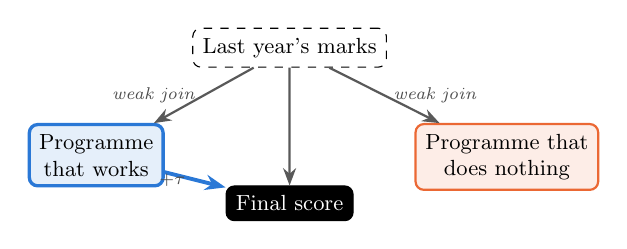
\begin{tikzpicture}[scale=0.88, transform shape, node distance=8mm and 4mm]
\node[hid] (p) {Last year's marks};
\node[cs, below left=of p] (x) {Programme\\that works};
\node[dc, below right=of p] (o) {Programme that\\does nothing};
\node[outc,below=17mm of p] (f) {Final score};
\draw[ar] (p)--node[lab,left]{weak join}(x); \draw[ar] (p)--node[lab,right]{weak join}(o); \draw[ar] (p)--(f);
\draw[arc] (x)--node[lab,left]{$+\tau$}(f);
\end{tikzpicture}
\caption{Level 3: Simpson's paradox.}\end{subfigure}\hfill
\begin{subfigure}[t]{0.49\textwidth}\centering
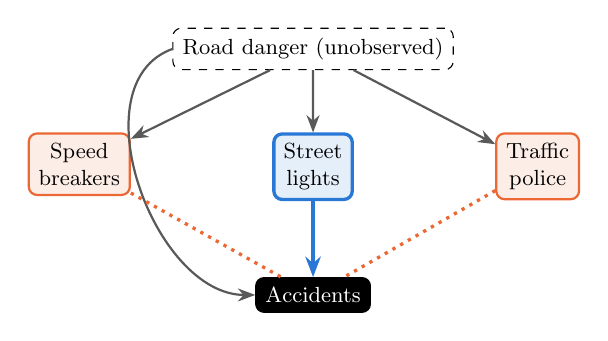
\begin{tikzpicture}[scale=0.88, transform shape, node distance=8mm and 2mm]
\node[hid] (d) {Road danger (unobserved)};
\node[dc, below left=9mm and 6mm of d] (a) {Speed\\breakers};
\node[cs, below=9mm of d] (b) {Street\\lights};
\node[dc, below right=9mm and 6mm of d] (c) {Traffic\\police};
\node[outc,below=11mm of b] (y) {Accidents};
\draw[ar] (d)--(a); \draw[ar] (d)--(b); \draw[ar] (d)--(c);
\draw[ar] (d.west) to[out=200,in=180] (y.west);
\draw[arc] (b)--(y); \draw[sp] (a)--(y); \draw[sp] (c)--(y);
\end{tikzpicture}
\caption{Level 4: unobserved confounder (cause shuffled).}\end{subfigure}
\caption{Hidden causal diagrams. Blue: the real cause; orange: the decoy; dashed box: the common cause; dotted line:
correlation without a causal arrow.}
\label{fig:dags}
\end{figure}

\paragraph{Level 1 (confounding).} Rainfall and temperature follow $S(t)$. Two breeding-site types are generated as
$\text{site}_{w,t} = d_w\,\text{rain}_{w,t}/10 + 0.8e$; only one of them (chosen at random) causes dengue. Ice-cream sales are
$\text{base}_w + k(\text{temp}_{w,t}-25) + 1.5e$. The town records \emph{complaints}, $\text{round}(\rho_w\,\text{site} + 1.5e)$,
with a ward-specific reporting rate $\rho_w$. Dengue is
$\text{Poisson}\big(b_0 + \beta\,\text{site}^{\text{cause}}_{w,t-2}\,(\text{temp}_{w,t}-20)/10\big)$.
Ice-cream has no arrow into dengue; both share the season.

\paragraph{Level 2 (reverse causation).} Fever is $\text{Poisson}\big(a\,\kappa_w\,(0.4+S(t))\,e^{-\gamma\,\text{clinics}_{w,t-1}}\big)$
with hidden ward risk $\kappa_w$ and $\gamma\in[0.05,0.09]$. The town opens a clinic (probability 0.2--0.3 per week) whenever the
previous four weeks averaged above a threshold, so fever causes clinics while clinics reduce fever. Pharmacy sales are
$20 + 3.5\,\text{fever} + 4e$, caused by fever.

\paragraph{Level 3 (Simpson's paradox).} For each student, prior marks are $N(55,16)$ and define a Low/Mid/High group.
Enrolment probabilities are 0.75--0.90 (Low), 0.20--0.35 (Mid) and 0.04--0.10 (High). The final score is
$8 + 0.9\,\text{prior} + \tau_A A + \tau_B B + 8e$, where one of $\tau_A,\tau_B$ is drawn from $[6,10]$ and the other is 0.

\paragraph{Level 4 (unobserved confounder).} A hidden danger $\delta_w\in[0.6,1.6]$ drives traffic (only partly), the placement
of three candidate measures, and accidents, $\text{Poisson}\big(b\,\delta_w\,(0.7+0.6S(t))\,e^{-\theta(X^{c}_w-\bar X^{c})}\big)$.
Exactly one measure $c$ (shuffled) has $\theta>0$, calibrated so a full roll-out cuts accidents by 25--40\%.

Level~5 reuses the models of Levels~1, 2 and 4 with new variables and stories (diarrhoea and cold drinks; thefts and police
posts; school absence with buses, meals and uniforms).

\subsection{Fresh worlds and rejection sampling}
Every game draws new parameters, ward traits and, where possible, the role of each candidate (which site type, programme or
road measure is the real cause). A world is accepted only if it contains the level's trap, which is checked on the
generated data (Table~\ref{tab:traps}); otherwise it is redrawn from the same seeded stream. For the confounding levels the
check also requires the trap to be \emph{beatable}: on ward yearly averages, where the shared season cancels out, the real
cause's complaints must track the outcome ($r>0.4$) and clearly beat the decoy. The noise levels were tuned so that most raw
worlds already satisfy the check (Table~\ref{tab:valid}), so players see typical worlds rather than rare, cherry-picked ones.

\begin{table}[H]
\centering\small
\caption{Trap conditions checked on every generated world.}
\label{tab:traps}
\begin{tabularx}{\textwidth}{@{}P{2.6cm}L@{}}
\toprule
Level & Accepted only if \\
\midrule
Confounding & decoy is the strongest ward-week correlate ($r>0.5$, beating both complaint series by $\ge 0.05$); on ward averages the cause has $r>0.4$ and beats the decoy and the other site by $\ge 0.25$ \\
Reverse & ward-average $r(\text{clinics},\text{fever})>0.4$; in the event study fever is $>115\%$ of the ward's usual level in the 3 weeks before a clinic opens, and rising \\
Simpson & real programme's attenders score $>3$ marks lower overall but $>1.5$ marks higher in every group; the useless programme also looks worse overall \\
Unobserved confounder & all three measures have ward-average $r>0.2$ with accidents, and the strongest is not the real cause \\
\bottomrule
\end{tabularx}
\end{table}

\subsection{Interventions and common random numbers}
All randomness for the coming season is drawn once, when the world is generated. Every policy, and the no-policy baseline,
is simulated on exactly these numbers, so the difference between the two runs is the policy's effect and nothing else.
Poisson counts are obtained by inverse-CDF sampling from stored uniforms, so a policy that leaves an outcome's rate unchanged
produces identical counts: interventions on non-causes have an impact of \emph{exactly} zero, which the tests verify.

\subsection{The randomised pilot}
A pilot assigns the policy to 10 of the 20 wards by a seeded random permutation, for 4 weeks of the actual simulated season;
the remaining weeks are left for the roll-out, so a pilot costs both money (Rs.~5 lakh) and time. Each ward's mean outcome during
the pilot is divided by its own last-year average, which removes fixed differences between wards, and treated and control wards
are compared with Welch's two-sample $t$ interval:
\begin{equation}
\hat\Delta = \bar y_T - \bar y_C,\qquad \hat\Delta \pm t_{0.975,\nu}\sqrt{s_T^2/n_T + s_C^2/n_C},
\end{equation}
with Welch--Satterthwaite degrees of freedom $\nu$. Because the assignment is random, the unobserved danger is balanced
between the groups in expectation, so $\hat\Delta$ estimates the causal effect.

\subsection{Reproducibility}
Random numbers come from a seeded generator (mulberry32). The seed is shown on screen; entering it rebuilds the identical
town, data, pilot assignments and outcomes. Decorative graphics use a separate random stream and never affect the simulation.

\section{Implementation}
The game is plain HTML, CSS and JavaScript with no build step, libraries or network access, so it runs by opening
\texttt{index.html} and can be hosted on GitHub Pages unchanged. Scripts are classic \texttt{<script>} files rather than ES
modules because browsers block modules on \texttt{file://} pages. All charts, the town and the causal diagrams are drawn
in SVG. Table~\ref{tab:modules} lists the modules; the simulation files are shared verbatim between the browser and the
Node.js tests.

\begin{table}[H]
\centering\small
\caption{Code organisation.}
\label{tab:modules}
\begin{tabularx}{\textwidth}{@{}P{4.3cm}L@{}}
\toprule
Module & Responsibility \\
\midrule
\texttt{rng.js}, \texttt{stats.js} & Seeded PRNG, Poisson from a given uniform; mean, SD, Pearson $r$, Welch interval, event study \\
\texttt{scm/common.js} & Rejection sampling, common-random-numbers evaluation, phased plans, pilot analysis, scoring \\
\texttt{scm/l1}--\texttt{l4} & The four causal models, each with re-themed Level 5 variants \\
\texttt{levels.js} & Stories, tools, causal diagrams and explanations generated from each world's numbers \\
\texttt{charts.js}, \texttt{town.js}, \texttt{fx.js} & SVG charts, the data-driven town, animations \\
\texttt{ui.js}, \texttt{quiz.js}, \texttt{log.js} & Screens and game loop, pre/post quiz, decision logging and export \\
\texttt{tests/sim.test.js} & 44 automated tests (\texttt{node -{}-test}) \\
\texttt{tools/} & Log summariser (Python) and validation statistics (Node) \\
\bottomrule
\end{tabularx}
\end{table}

\paragraph{Usability and accessibility.} The layout adapts to phone screens; the town and diagrams scroll inside their
cards on narrow screens. Chart colours come from a colour-blind-checked categorical palette, every series is labelled
directly, and colour is never the only cue (icons and numbers accompany it). The game uses a single night-time visual
theme, ``Navapuram at dusk'': a silhouette skyline of the town, headings styled like painted signboards, a treasury of
rupee coins for the budget, and one accent colour per concept taken from its story. All animations are disabled when the
device requests reduced motion.

\section{Validation}
\subsection{Automated tests}
The 44 tests run in about three seconds with plain Node.js. For every model (including the three Level~5 variants) they check
that worlds are replayable from their seed, that the trap holds in 150 generated worlds, that rejection sampling needs few
tries, and that the real cause is shuffled. They further check that interventions on non-causes have exactly zero impact,
that harmful policies harm and the best policy is best, that a pilot plan's impact lies between doing nothing and a full
roll-out, and that the statistical helpers reproduce reference values (Pearson $r$, $t$ quantiles, Welch interval).

\subsection{Model behaviour}
Table~\ref{tab:valid} reports statistics over fixed seeds, produced by \texttt{tools/validation\_stats.js}. In all 2{,}400
checked interventions on non-causes the impact was exactly zero.

\begin{table}[H]
\centering\small
\caption{Validation statistics (500 raw worlds per model for the trap rate; 200 accepted worlds for the rest).}
\label{tab:valid}
\begin{tabularx}{\textwidth}{@{}LP{2.3cm}P{2.3cm}P{4.1cm}@{}}
\toprule
Model & Raw worlds with trap & Mean generation tries & Best policy's impact (\% of the no-policy outcome) \\
\midrule
L1 dengue (confounding) & 71.2\% & 1.43 & 57.5\% fewer cases \\
L2 clinics (reverse causation) & 96.6\% & 1.01 & 11.7\% fewer cases \\
L3 coaching (Simpson) & 99.0\% & 1.01 & 3.3\% more total marks \\
L4 roads (unobserved confounder) & 25.8\% & 3.31 & 28.8\% fewer accidents \\
L5a diarrhoea (confounding) & 68.8\% & 1.40 & 57.3\% fewer cases \\
L5b thefts (reverse causation) & 96.8\% & 1.06 & 11.6\% fewer thefts \\
L5c school (unobserved confounder) & 43.0\% & 2.15 & 29.7\% fewer absences \\
\bottomrule
\end{tabularx}
\end{table}

\noindent The lower raw rate for the unobserved-confounder levels is expected: the trap requires the strongest correlate not
to be the cause, which holds by chance in about two thirds of draws before other conditions. Over 300 worlds per model,
the pilot estimate was unbiased (mean error $-0.006$ for roads, $-0.009$ for school absence, on the relative scale), its 95\%
interval contained the true effect in 94.7\% and 90.3\% of pilots respectively, it identified the real cause (interval below
zero) in 88.7\% and 88.0\% of pilots, and for non-causes the interval contained zero in 94.0\% of pilots. The slightly low
coverage for school absence reflects the small groups (10 wards each) and is accepted as realistic: a pilot is informative
but not infallible.

\section{Evidence of learning}
\subsection{Instruments}
Three instruments are built into the game. (i) A \textbf{decision log} records, for every problem, the policy chosen, cost,
pilots run, true and best impact, whether the player fell for the trap or picked the real cause, the score, time spent
exploring, tools opened and whether the level's key tool was used; it also records exploration events. (ii) An optional
\textbf{scenario quiz} of three questions (confounding, reverse causation, randomisation) is taken before Level~1 and an
equivalent set with different scenarios after Level~5. (iii) A \textbf{feedback form} collects a 1--5 helpfulness rating and
two free-text answers. The player downloads all of this as a JSON or CSV file. The script \texttt{tools/summarize\_logs.py}
combines players' logs into a per-player table, a summary of trap-fall rates (Level~1 against the same trap type in a new
story in Level~5), pre- versus post-quiz scores and ratings, and a chart.

\subsection{Playtest protocol}
Each peer plays once with a player tag and no help while an observer notes hesitations and comments, takes both quizzes,
completes the feedback form and sends the downloaded log. The protocol and an observation template are in
\texttt{docs/playtest/}.

\subsection{Results}
\textbf{Developer walkthrough.} An end-to-end run by the developers (Firefox, seed 478836) completed all seven problems,
both quizzes, the feedback form and the log export without errors. As expected for players who built the game, the quiz
scored 3/3 both before and after; this run is a functional check and is not counted as evidence of learning.

\textbf{Peer playtests.} Peer playtest sessions were not conducted within the project timeline. The instruments
described above are complete and tested end to end: running the protocol with a group of players produces the trap-fall
comparison, the pre/post quiz comparison, the ratings and the comments without further development.

\section{Limitations and future work}
\begin{itemize}
  \item The models are deliberately simple and stylised; real epidemiology, education and traffic systems have many more
  causes, feedback loops and measurement problems.
  \item Only one policy is funded per problem, and policies do not interact; combining policies would allow richer reasoning.
  \item The pilot uses a fixed design (4 weeks, 10 versus 10 wards). Letting players choose its size would teach the trade-off
  between precision and cost.
  \item The developer walkthrough showed that the warm-up quiz can reach a ceiling for players who already know the slogan;
  harder distractors and shuffled answer order would make pre/post comparisons more sensitive.
  \item Learning gains have not yet been measured with peer players; the instruments and protocol for that study are in place, and with a small group the result would be descriptive rather than a controlled study.
\end{itemize}

\section{Conclusion}
\emph{Mayor for a Year} turns ``correlation does not imply causation'' into a sequence of decisions with visible
consequences. Because the town is a structural causal model, the game can show every player the true effect of their
choice next to the correlation that tempted them, and the hidden diagram that explains the difference. Fresh, seeded worlds
with verified traps keep the answers from being memorised, common random numbers make the true impact exact, and the
randomised pilot lets players experience why an experiment settles what observational data cannot.

\appendix
\section{Running the game and the tests}
\begin{itemize}
  \item Play: open \texttt{index.html} in a modern browser (offline), or run \texttt{python -m http.server} in the folder.
  \item Tests: \texttt{node -{}-test} (Node.js 18 or newer, no packages).
  \item Validation statistics: \texttt{node tools/validation\_stats.js}.
  \item Playtest summary: place the logs in \texttt{docs/playtest/logs/}, then run\\ \texttt{python tools/summarize\_logs.py}.
\end{itemize}

\begin{thebibliography}{9}
\bibitem{pearl} J.~Pearl, M.~Glymour and N.~P.~Jewell, \emph{Causal Inference in Statistics: A Primer}. Wiley, 2016.
\bibitem{hernan} M.~A.~Hern\'an and J.~M.~Robins, \emph{Causal Inference: What If}. Chapman \& Hall/CRC, 2020.
\bibitem{simpson} E.~H.~Simpson, ``The interpretation of interaction in contingency tables,'' \emph{Journal of the Royal Statistical Society, Series B}, vol.~13, no.~2, pp.~238--241, 1951.
\bibitem{fisher} R.~A.~Fisher, \emph{The Design of Experiments}. Oliver and Boyd, 1935.
\bibitem{welch} B.~L.~Welch, ``The generalization of `Student's' problem when several different population variances are involved,'' \emph{Biometrika}, vol.~34, no.~1--2, pp.~28--35, 1947.
\bibitem{law} A.~M.~Law, \emph{Simulation Modeling and Analysis}, 5th ed. McGraw-Hill, 2015 (common random numbers).
\end{thebibliography}
\end{document}
